\documentclass[11pt]{article} % do not change this line
\input{BigDataStyle.txt}      % do not change this line

\usepackage{amsmath,amsfonts,amssymb,amsthm,latexsym,graphicx,caption,hyperref,listings,color,xcolor}
\usepackage[export]{adjustbox}
\usepackage{float} 
\usepackage[section]{placeins}
\usepackage[boxed,ruled,vlined,dotocloa,english,onelanguage]{algorithm2e}
%\graphicspath{ {pictures/} }
\emergencystretch=5mm
\tolerance=400
\allowdisplaybreaks[4]


\theoremstyle{plain}
\newtheorem{theorem}{Theorem}[section]
\newtheorem{proposition}[theorem]{Proposition}
\newtheorem{corollary}[theorem]{Corollary}
\newtheorem{lemma}[theorem]{Lemma}
\newtheorem{problem}[theorem]{Problem}

\theoremstyle{definition}
\newtheorem*{remark}{Remark}

\title{Key Management for the Interplanetary Internet}
\author{Marcos Tileria}

\newcommand{\Programme}{Doctoral Training Centre in Cyber Security}


\begin{document}
\maketitle

\declaration

\begin{abstract}

  
The Interplanetary Internet is a conceived computer network designed to provide Internet-like services to space missions. Communication in deep space is characterised by extremely long delays and the lack of end-to-end connectivity. Security is a principal component of the Interplanetary Internet. Cryptography key management is considered one of the most difficult security problems for space-based networks, and there is no widely accepted solution to this problem. This project provides an evaluation of the so far proposed key management solution.   


  
\end{abstract}



\section{Introduction}


Different research groups
experiments
why no tcp and others
other protocols: LTP, CFDP, 
security

Cryptographic Key Management is recognised as the most difficult problem in DTNs. For many years, research and working groups from IETF and other organisation left the problem unsolved and assumed that there was a reasonable key management solution that can be used to generate, update and distribute keys among DTN nodes. 

Key management is a central part of any secure communication system and plays a critical role in overall security. Furthermore, key management is recognised as a difficult problem in a connected network, and a disrupted network subject to long delays make the problem even more complicated.  


The future space exploration envisions multiple space nodes that communicate with each other and not only between space and Operation Centre (OC). A space node could be any human-made object send into deep space in support of space mission, for instance, satellites, orbiters, landers, rovers or any small robot. An immediate consequence of the new communication model will be an increase in the number of interconnected systems, data transfer and connectivity. The current architecture is not designed to support such expansion, and an upgrade will be necessary. A similar situation occurred in the early days of telephone systems and switchboards. As the number of users grew, it was not possible human circuit switching anymore, and the system had to evolve into an automated switching systems \cite{rationale2010requirements}. The space communication architecture requires a transformation from point-to-point communications toward a flexible architecture capable of managing the new communication requirements of future space missions. 


 \newpage

\section{Deep Space Communications}
\label{sec:space}

There are significant differences between space-based communications and traditional communications on Earth. The physical properties of deep space are fundamental at the time of design communication protocols. This section gives a review of the principal components of space-based communications, the evolution of the communication model in space missions and provides an overview of the current security measures in space communication. 


\subsection{Space-based communications}

The launch of the Sputnik 1 satellite in 1957 gave origin to the Space Race. Human spaceflights and unmanned robotic space probes were developed to support space exploration. Communication systems were designed to send commands from a mission control centre (telecommand) and receive telemetry or science data from spacecraft. The original idea was simple: the mission control centre sends a radio frequency signal to a spacecraft, then the spacecraft receives the signal via its antenna and process the telecommand. Finally, the spacecraft replies with telemetry commands or science data if requested to do so. A simplified diagram of a space mission architecture is shown in the figure \ref{fig:space-based-arc}.  

%As exploration mission went farther away in the solar system or requiere more science data from spacecraft, communication systems had to evolve to keep the pace of space missions complexity.


\begin{figure}[ht]
\centering
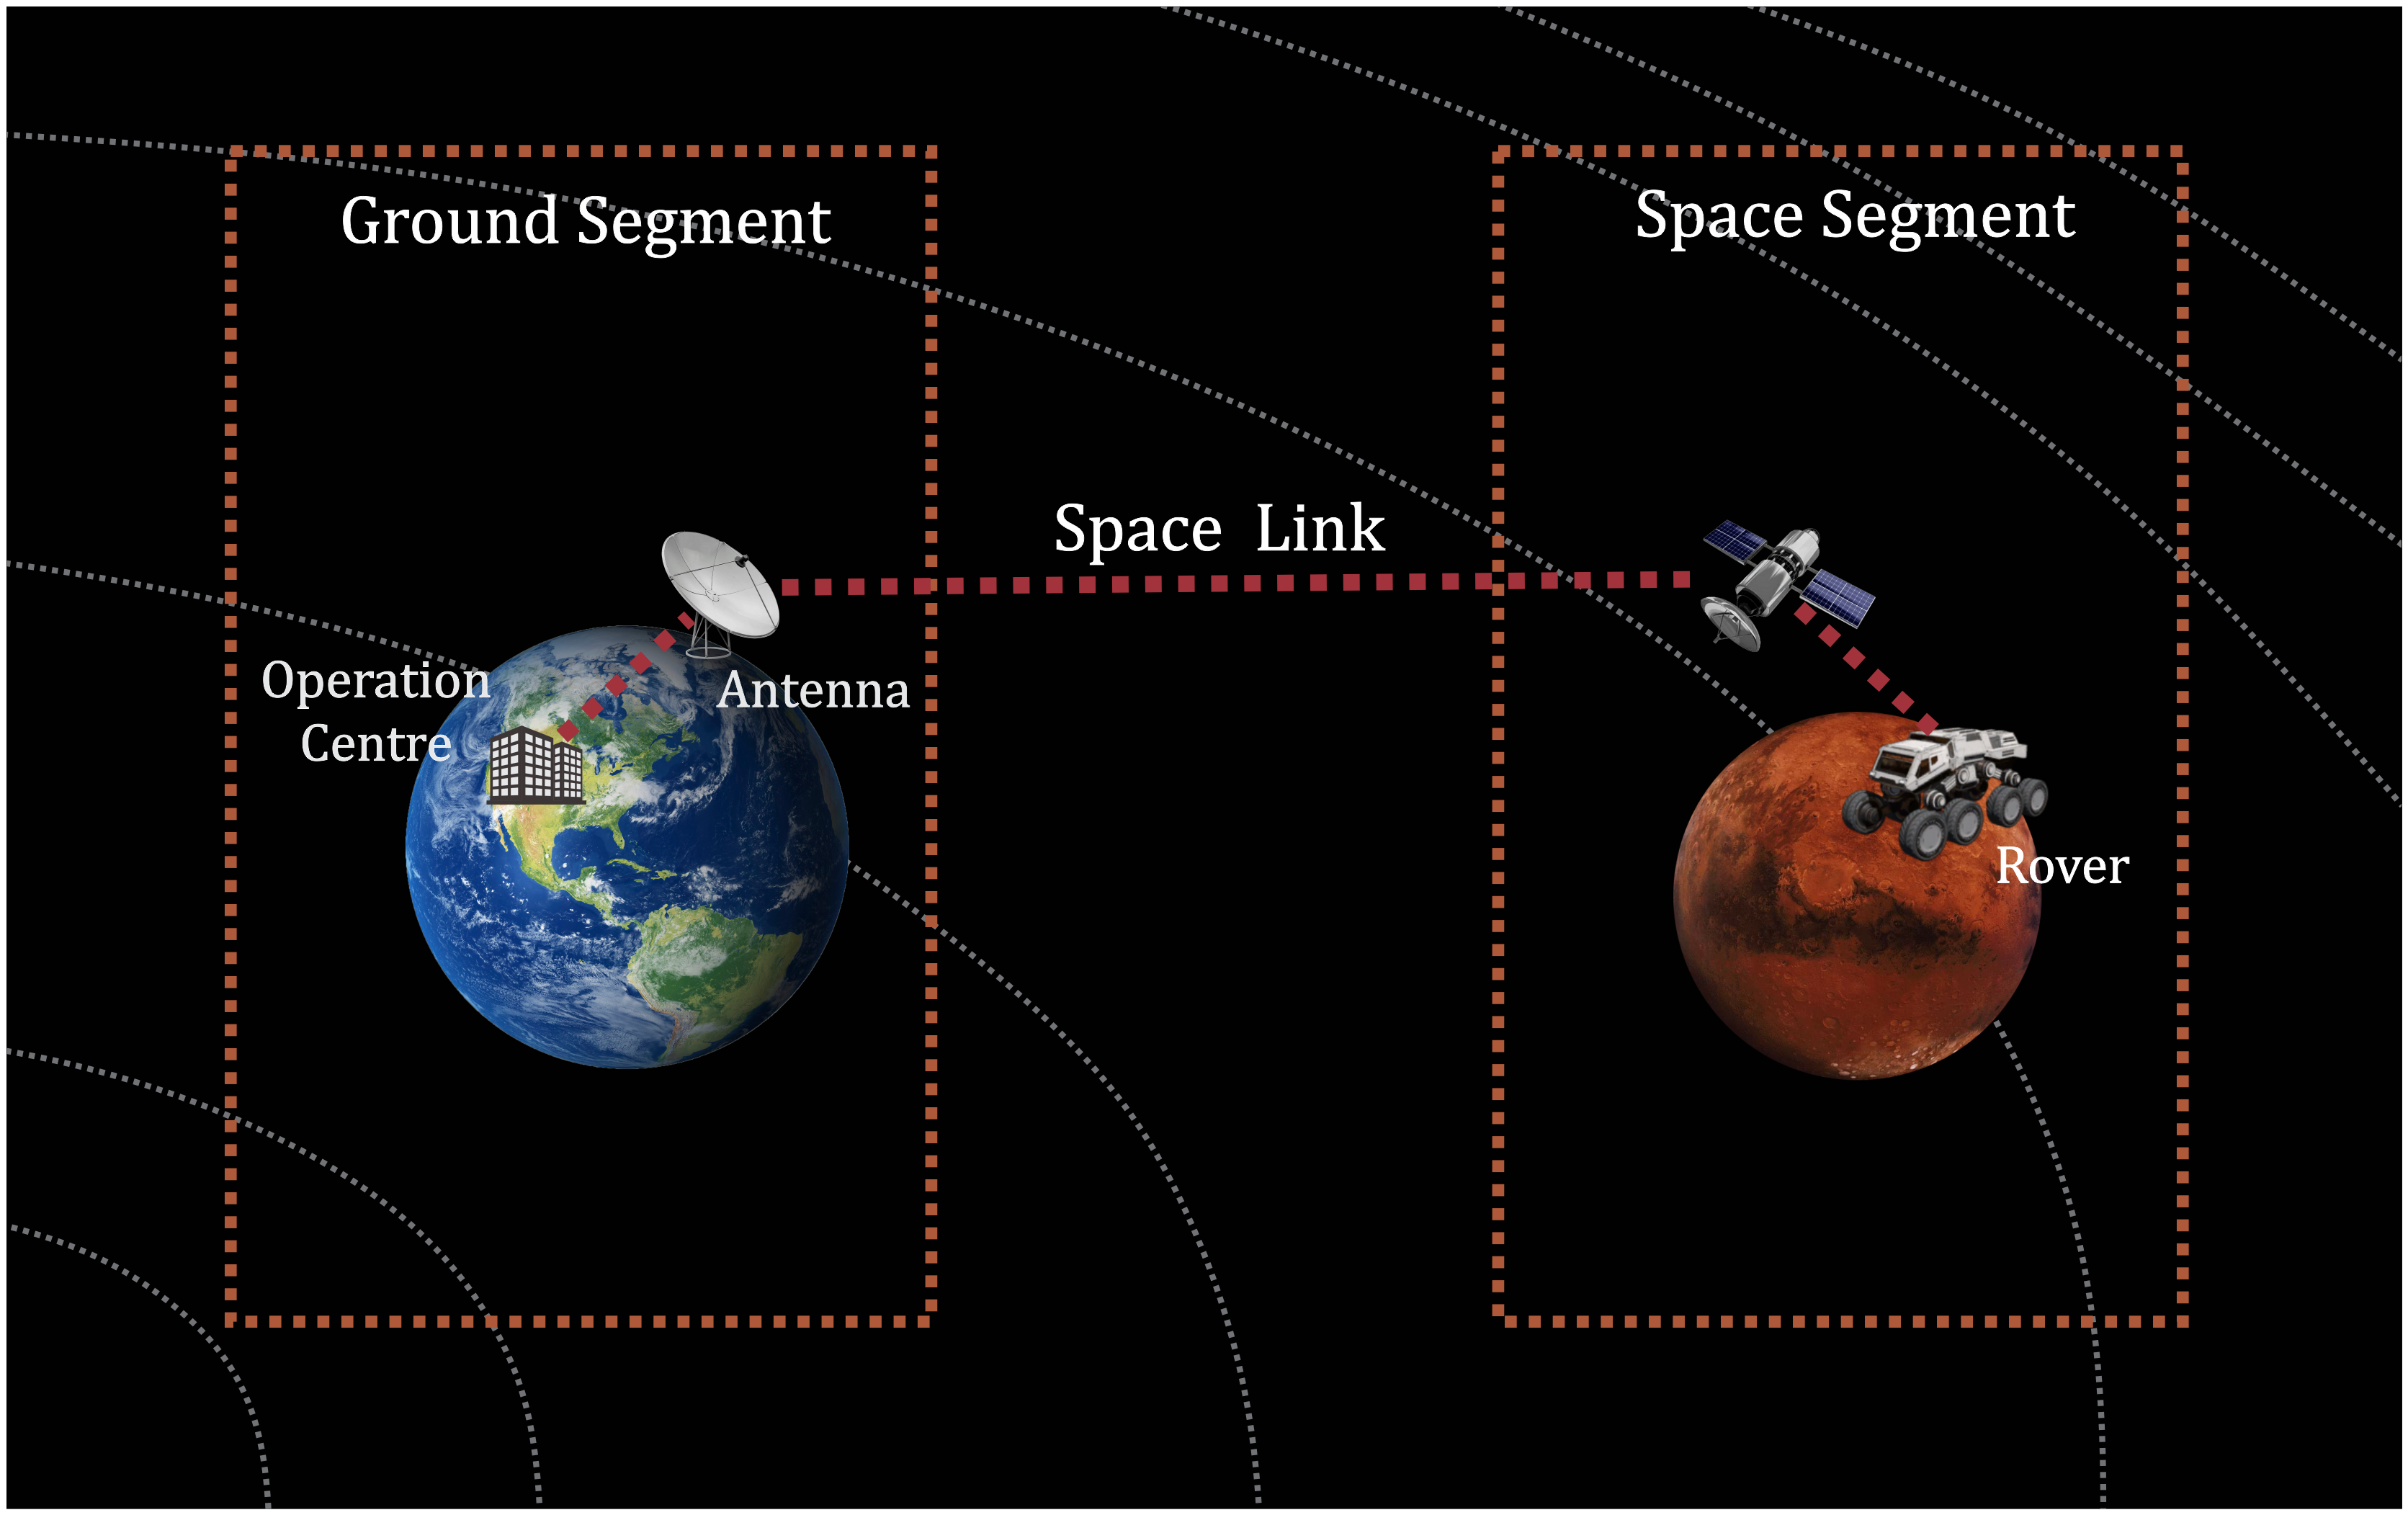
\includegraphics[width=1 \linewidth, height=9.5cm]{images/ground.png} 
\caption{Space-based communication architecture}
\label{fig:space-based-arc}
\end{figure}

In this example, the satellite and the Mars rover form part of the space segment. The space-link is the connection between the ground station and the satellite.  The ground station and the mission control centre constitute the ground segment. The mission control centre, sometimes called Operational Control Centre (OCC) has the control of the objects in deep space. This example shows the most complex scenario which is currently deployed in the Mars Exploration Rover mission \cite{crisp2003mars}. In the vast majority of space missions, the communication is directly between the OCC and the end-point in the outer space.

 The most significant differences between space-based and terrestrial communications are the long propagation delay due to the speed of light and the lack of end-to-end connectivity caused by planets motion. The result is disrupted communication subject to significant propagation delays. These inherent space properties make well-known protocols for terrestrial networks unsuitable for space communications \cite{fall2003delay}.


The distance of a space object to the earth determines the type of the communication. Near-earth communications present low delay and intermittent connectivity. Satellites in geosynchronous orbit are subject to low delay but continuous connectivity. Earth-Moon communication is a particular case, the round-trip delay is approximately 2.5 seconds, and there is a disruption in the communication due to the motion of the Earth and the Moon. Space missions beyond the Moon present the worst case: extremely long propagation delay and disrupted communication. For instance,  a signal from the farthest human-made object in deep space (Voyager 1) takes over 19 hours to reach the Earth. Signals sent by Mars rovers take between 7 and 20 minutes to reach Earth, depending on the position of the planets. 
% Moreover, a rover has to be in line-of-sight of an orbiter or the Earth to send or receive data, producing disrupted communication  



Physical limitations are not the only problem; the communication model presents problems as well. Firstly,  the communication infrastructure was designed to be point-to-point. Secondly, each mission operates independently and the cooperation between missions is almost nonexistent.  Therefore, many missions use bespoke communications protocols; a space mission typically focuses its resources on immediate problems, and subsequent missions have to ``reinvent the weel'' \cite{burleigh2003interplanetary}. 

However, over the last years, the situation is changing, and the Mars Exploration Rovers missions is an example. Besides, there is an effort from CCSDS and other bodies like IETF to standardised communication protocols for space missions. Examples include Space Packet Protocol and the Bundle protocol version for space communication, both developed by CCSDS. The Licklider protocol, developed by IETF, is a point-to-point protocol for use in deep space links.   % \cite{standard2010ccsds}. 

The relay mechanism employed in Mars was the first advance towards a packet-switched network style; however, there is no proper inter-networking yet under this configuration. Mars rovers use available orbiters as intermediate hops, but there is no addressing scheme, no classes of data and no proper network layer. These limitations will restrict operations of future missions which will require more communication capabilities \cite{rationale2010requirements}. 


The experience in Mars has shown the advantages of multi-hop communication over point-to-point communication. For instance increase in science data return, lower power and hardware requirements, and more contact opportunities \cite{rationale2010requirements}.  Besides, interoperability and cross-support across space agencies will be the usual situation in future space missions. Spacecraft, satellites, rovers and other human-made objects will operate as a network of space-based entities, similar to the figure \ref{fig:inter-internet}. 



\begin{figure}[ht]
\centering
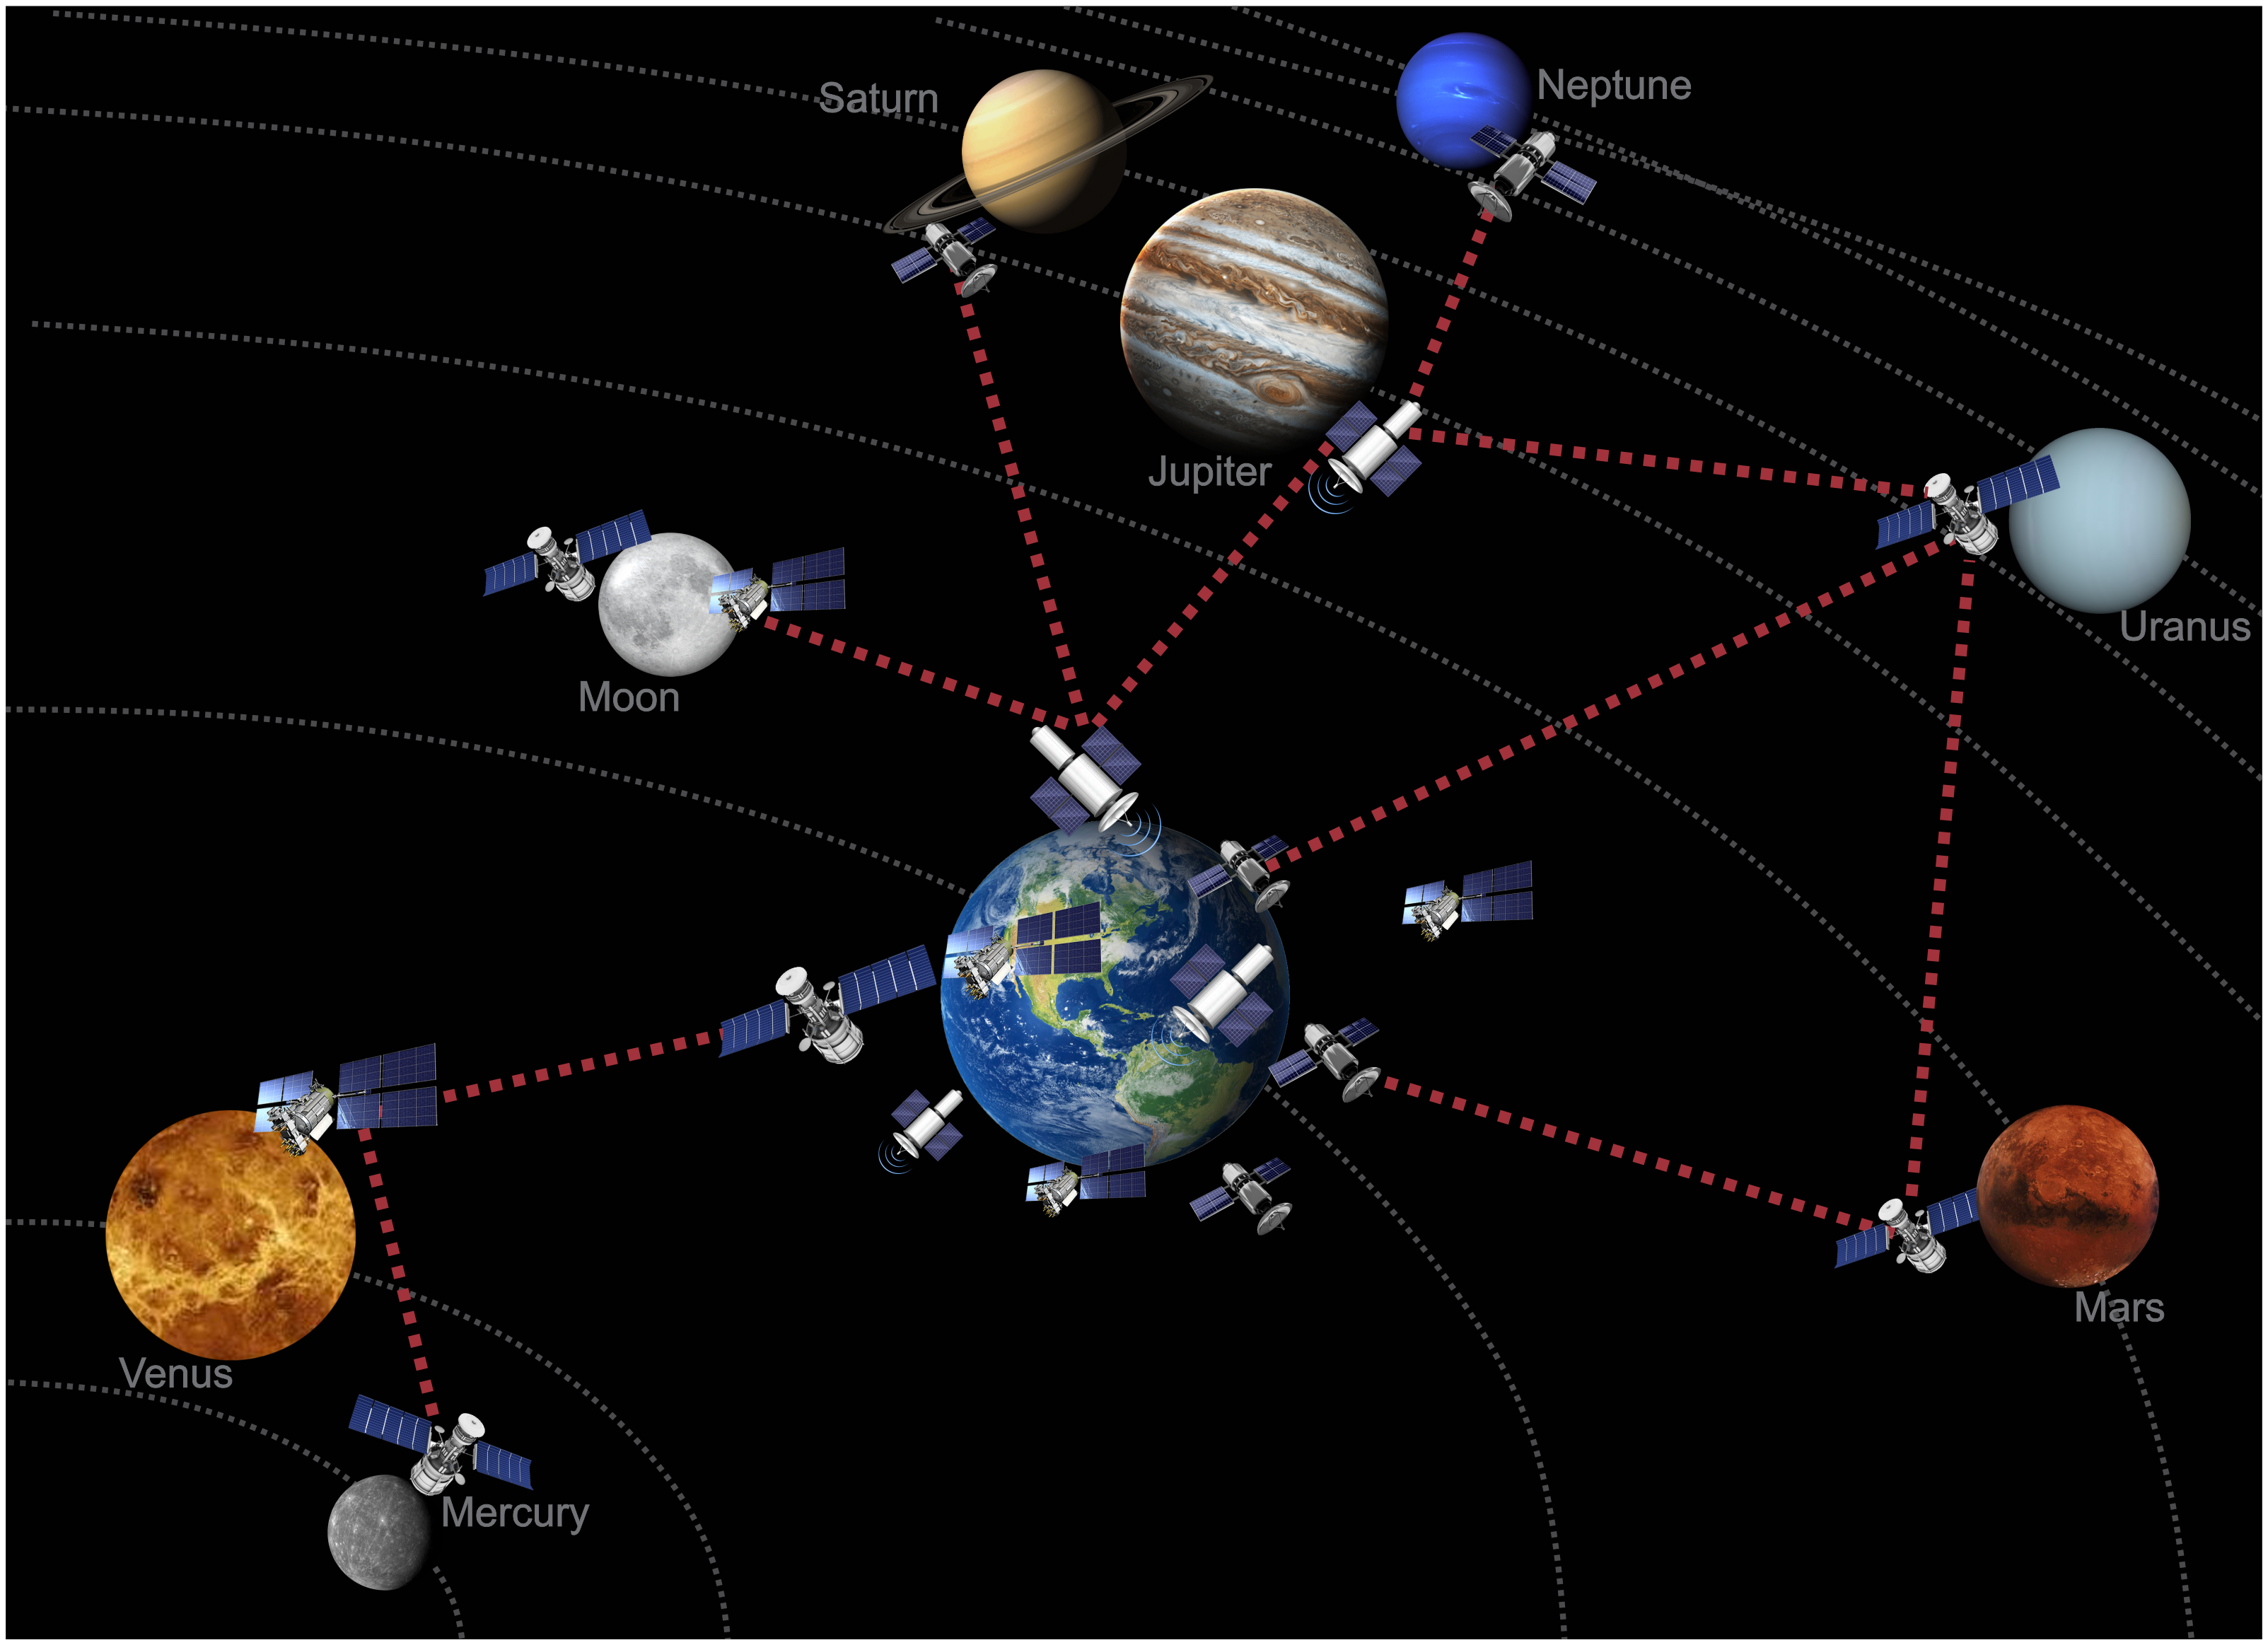
\includegraphics[width=1 \linewidth, height=9.5cm]{images/interplanetary.png} 
\caption{Interplanetary Internet}
\label{fig:inter-internet}
\end{figure}


\subsection{Security in Space Communications}


Cyber threats apply to all kinds of information systems, especially the ones administrated by nation-states. Space systems are becoming more interconnected to terrestrial systems and space missions are now target of malicious attackers.  In the past, only military missions were highly protected, but nowadays all types of missions require a certain level of security \cite{book2006security}.

Threats could apply to any segment of a space mission, space segment, ground segment or space-link. The diagram \ref{fig:space-based-arc} illustrates two important points which affect the overall security.  Firstly, the mission control centre and the ground station are not in the same physical location, and the link between them requires a secure connection, consequently key management. Secondly, the network infrastructure on the earth could belong to one entity and the mission control centre to another.  For instance, the  Mars Exploration Mission operates Mars rovers, but the Deep Space Network controls the communications Earth-Mars.

Point-to-point space links have been secured using bulk encryption \cite{book2011space}. Although this type of encryption is simple, it requires special techniques and hardware to be deployed on both ends of the space-link. However, bulk encryption is not scalable, multi-hop communication and interoperability among space agencies exclude bulk encryption as a candidate for the Interplanetary Internet %Ivancic \cite{ivancic2009security} mention potential problem in the US for international interoperability because The International Traffic in Arms Regulations might have jurisdiction.

The CCSDS published a report on security threats against space missions \cite{book2006security}. Adversaries include terrorist, criminals, foreign intelligence services, computer hackers, and commercial competitors.  Examples of active threats are jamming, unauthorised access, masquerading, Denial of Services. Passive threats could be tapping and traffic analysis.  The document states that security for space systems should be considered in the same way as any other information system.

 

% This situation suggests that security for the Interplanetary Internet should consider interoperability not only between nodes from different agencies, but it should consider interoperability between the Internet and space segment protocols. 

 %In \cite{book2012architecture}, CCSDS present security requirements for five space mission profile. These profiles are human spaceflight, earth observation, communication, scientific, and navigation. For instance, humans spaceflights present all security requirements but also ``safety-of-life'' and privacy issues. The security of earth observation, navigation, and communications missions vary depending on the information value and the relative position to the earth. Some missions require security for telemetry, telecommands, and payload communication, others only need to secure a subset of those. 
 
 %These profiles are human spaceflight, earth observation, communication, scientific, and navigation. 
CCSDS presents different mission profile for space missions \cite{book2012architecture}. Some mission profiles require security for telemetry, telecommands, and payload communication; others only need to secure a subset of those. Human spaceflights are especially sensitive, but science missions present the most difficult scenarios as spacecraft might be exploring remote locations in the solar system and in general, missions lifetime are significantly longer. In multi-organisational missions, hardware, payloads and data may belong to different space agencies. Relay satellites and endpoints might be administrated by different space agencies as well.

For many countries, satellites already form part of critical infrastructures like navigation, weather study, and disaster response \cite{book2006security}.  As state before, future missions will require interoperability between space nodes that might be administrated by different agencies. Therefore, space mission planners must consider the implementation of secure communications protocols whether the nodes are in orbit around Earth or exploring remote places in the solar system.


 
 %For instance, humans spaceflights present all security requirements but also ``safety-of-life'' and privacy issues. The security of earth observation, navigation, and communications missions vary depending on the information value and the relative position to the earth. 
 
 %Science missions are more complicated than the previous,  the distance to the earth change requirements dramatically. For interplanetary missions, there are extra factors that should be considered at the time of implementing security, for instance, communication delay, discontinuous communication, fault tolerance, ability to use intermediate nodes (planned and unplanned), significant mission lifetime. The last point to consider is 
 
 %A clear example is optical communications in space, state of the art techniques are not competitive in mass and power performance against radio frequency RF communication, and there are several projects ongoing to meet the performance goals required by mission planners. It remains to see how different profiles could fit in a single key management scheme.
 



\subsection{Key Management in current Missions}

In current space missions, key management complexity is low.  Typically, the mission control centre and spacecraft are the entities involved. The mission control centre is responsible for generating, managing and revoking keys. For human-crewed missions, the human intervention in key management operations is limited. Optionally, the ground station could take part in key management operation if it is working as a security gateway.  User facilities may be present if payload data have to be disseminated \cite{book2011space}. 


Commonly keys are stored in smart cards in physical protected places. Key generation procedure affects only the ground segment. Master keys are used to generate or exchange new keys of lower hierarchy such as traffic protection keys or key encrytion keys. In the case that a master key is used as an encryption key, all key management operations are conducted before launch. Any number of master keys could be used at the discretion of mission planners \cite{book2011space}.

Many environmental properties influence a key management solution in space missions. Asymmetric channels, bandwidth restriction, propagation delay, intermittent connectivity, remote locations. All these constraints apply to communication and cryptographic protocols, but limited computational resources and memory should be considered for key management as well. For instance, some nodes might not be able to perform cryptographic operations, and the memory size limits the information that a node can store like keys or revocation list.

Although these limitations imply that symmetric key cryptosystems are more suitable for space missions \cite{book2011space}, future space missions present a different scenario and it is unlikely than symmetric cryptosystems fit the requirements mention before for the Interplanetary Internet.

%It is likely to have group key management for multicast within the network.  


 \newpage

\section{Bundle Protocol and Security Specifications}
\label{sec:dtn}

The Delay Tolerant Networking RFC \cite{cerf2007delay} defines an architecture for irregularly connected networks subject to frequent partition and possibly long propagation delays. To face these particular properties, the authors propose an overlay layer, called the \textbf{bundle layer}, which provides end-to-end reliable messages delivery. This layer works over the transport, network or data link layer using different convergence layer to communicate with lower layer protocols. The Bundle protocol specification \cite{rfc5050} defines the services offered by the bundle layer, data processing format, bundle processing and convergence layers. 

\begin{figure}[ht]
\centering
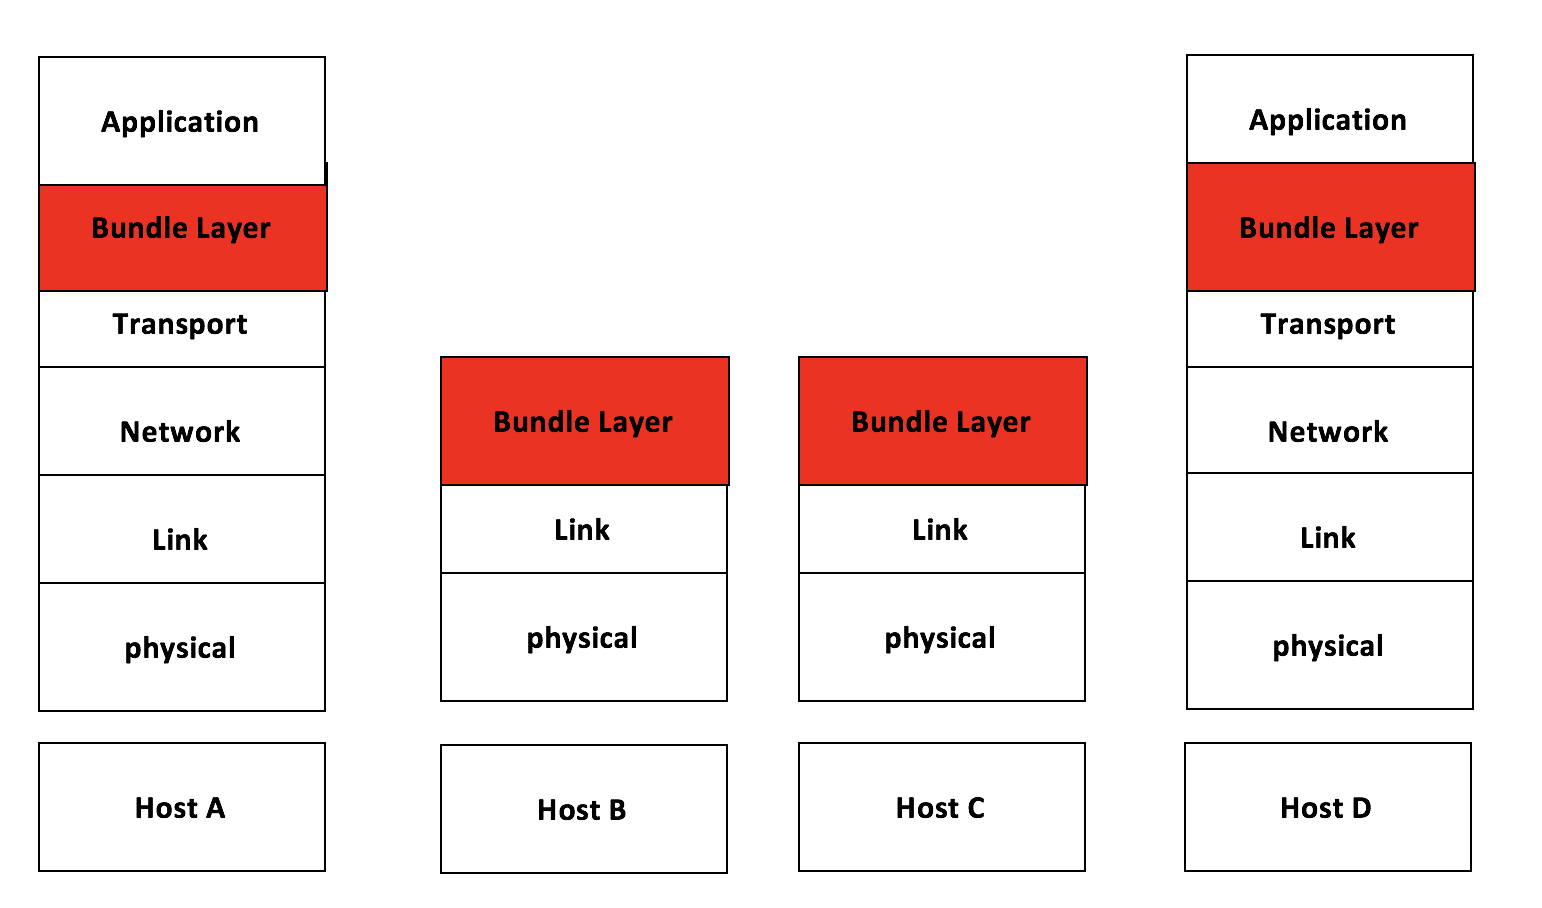
\includegraphics[width=1 \linewidth]{images/bundle.png} 
\caption{Bundle layer}
\label{fig:bundle}
\end{figure}

A bundle is the basic data unit of the Bundle protocol, similar to a packet for the IP protocol. A \textbf{bundle node}, DTN node or just simply a node could be any entity that can send or receive bundles; in other words, it is an implementation of the bundle layer. Note that a spacecraft could contain more than one instance of the Bundle protocol. For instance, the International Space Station is considered a network itself rather than a single bundle node. Negotiation between nodes might not be possible due to the delay and disruption, so a bundle is a self-contained data structure which has enough processing information.


The bundle layer provides persistent storage, hop-by-hop transfer, late binding, and optional end-to-end acknowledgement to overcome the constrained environment. The Bundle Protocol employs Universal Resources Identifiers (URI) as naming scheme, and this flexible model allows the encapsulation of different addressing schemes and late binding. 

According to CCSDS \cite{rationale2010requirements}, the Bundle protocol is the best-suited option to support in-space internetworking. There is ongoing work within the CCSDS to adapt and standardise the Bundle protocol and the security specifications. %The next section describes the security specification for the Bundle protocol. 

Many successful experiments of the Bundle protocol were already performed in deep space  \cite{ivancic2010experience}. The first experiment was conducted by Surrey Satellite Technology in 2008. The test consisted on deliver images taken by the UK-DMC Disaster Monitoring Constellation satellites to ground stations using the Bundle Protocol. Similarly, the NASA employed this protocol in the Deep Impact Space Network experiment for around four weeks on board the Deep Impact/EPOXI spacecraft. The International Space Station has been connected to the Internet since 2010 using the BP, and also performed many experiments with the NASA Jet Propulsion Labs. \cite{araniti2015contact}.    


\subsection{Security for space DTNs}


 %From the beginning, the Delay-Tolerant Research Group worked on the security specifications for the Bundle protocol. The motivation was to provide data integrity and confidentiality services to the bundle layer. As space missions are more connected to the Internet and the economic value of space assets are very high is comprehensible consider information security as a critical component of the communication system.
 
 
The Bundle Security Protocol \cite{rfc6257} provides the specifications for data integrity and confidentiality services to the Bundle protocol. The document defines the data structure to provide the security services as extension blocks. A new document, still in active development \cite{ietf-dtn-bpsec-07}, defines two types of security blocks: Block Integrity Block (BIB) and Block Confidentiality Block (BCB). Previous versions of the specification define an extra security block, the Block Authentication Block BAB which was intended to provide hop-by-hop authentication but was removed in the last version of the document.     
 

Unauthorised access is a major problem for space DTNs, especially in the space segment where resources are scarce and expensive. Denial of service (DoS) is another concern; attackers could take advantage of long delays to make DoS attacks more effective \cite{rfc6257}. Sections of a space-based DTN may be untrusted, requiring encryption of payload and maybe the bundle meta-data. In the deep space, traditional mechanisms are not adequate; online access to a certificate authority cannot be assumed, and negotiation-based protocols are unsuitable.
 
 
The bundle layer operates as an overlay network; thus any vulnerability in lower layers apply to the bundle layer \cite{rfc6257}. Correspondingly, the space DTN could take advantage of security in other layers. The Bundle protocol allows a mix of ``security-aware'' nodes and ``non-security-aware'' nodes within an application domain. The lack of physical resources or security being implemented in other layers are potential scenarios for this situation. 

%\subsection{Key Management for DTN in space}
In a multi-hop communication, intermediate nodes may verify the integrity of the bundles or decrypt them according to security policies. Security-aware-nodes thus may need the corresponding verification or decryption keys, even if they are not the final destination. Key management system must contemplate this situation to fulfil the BSP.

A trade-off between usability against security is always present. Security adds overhead, but the limited resources in the space segment requires to maintain bandwidth and storage overhead low; otherwise, mission planners will reject the system. \cite{book2012architecture}.

%The next section is a literature review of the so far proposed key management solutions for DTN in space.
Add end paragraph.

\subsection{Standardisation effort}

Even though DTN working groups have been working actively since 2007, a key management specification has been postponed, mainly for its complexity \cite{rfc6257,irtf-dtnrg-sec-overview-06,templin-dtnskmps-00}. The Bundle Security Specification assumes that nodes are already in possession of shared or asymmetric key. Farrell presents high-level requirements for key management \cite{farrell-dtnrg-km-00}, but this document does not establish concluding requirements for a solution. Farrel argues that solutions must employ well-known protocols and options for manual keying, pre-shared keys, and public keys must be considered. 

The first significant advance was a problem statement by Templin in 2014  \cite{templin-dtnskmps-00}. This Internet-Draft suggests that the solution involves some type of public key cryptography and states the need for an automated system for publication of certificates and revocation lists. Templin affirmed that the system must be designed to continue the operation in the presence of long delays and intermittent connectivity, and there is no key management system which satisfies the requirements. The author suggests the use of one-time keys, so each bundle is encrypted with a symmetric key encrypted by the destination public key.  

Another more detailed Internet-Draft was published by the same author one year later \cite{templin-dtnskmreq-00}. The document proposes nine requirements for key management and four design criteria. The next section examines these requirements in detail.

Viswanathan \cite{viswanathan-dtn-pkdn-00} enumerates the possible communication patterns, data structure, architectural elements, and trust relationships.  This Internet-Draft provides a high-level solution for key distribution and revocations using the publisher/subscriber pattern. This model seems to be the best option for key distribution, assuming a key management based on public certificates. 

Finally, a newly published document proposed the Delay-Tolerant Key Administration DTKA \cite{burleigh-dtnwg-dtka-01}, which is a system for key management intended for the use in space-based DTNs. An overview of this system is presented in the next section.










\newpage

\section{Evaluation of proposals}
\newpage

\section{Discussion and Challanges}

Interoperability with terrestrial networks
Data privacy and anonymity coul be handle at application layer
Applicability of different keys and policies. in space networks might be too complex to perform this types of management. 
%\newpage

\section{Conclusions}
%\newpage


\bibliographystyle{unsrt} %plain
\bibliography{bibliography}
\end{document}


